\section{Robust MPC}
\textbf{Uncertain constrained linear system}
\[ \boxed{x(k+1) = A x (k) + Bu(k)+w(k)\hspace{5mm} x,u \in \mathcal{X,U} \hspace{4mm}w\in \mathcal{W}}\]
\textbf{Goal:}
Design control law $u(k)= \mathcal{K}(x(k))$ such that the system: 
\begin{itemize}
    \item satisfies constraints : $\{x(k)\} \subset \mathcal{X}, \{u(k)\} \subset \mathcal{U} \forall$ disturbance realizations 
    \item Is stable: Converges to a \textbf{neighbourhood} of the origin
    \item optimizes (Expected/worst-case) "performance"
    \item Maximizes the set $\{x(0)|\textrm{Conditions 1-3 are met}\}$
\end{itemize}
\subsection{Defining a Cost to Minimize}
    Cost as a function of the disturbance seen:
    \[J(x_0,U,W) := \sum^{N-1}_{i=0} I(\Phi_i(x_0,U,W),u_i) + I_f(\Phi_N(x_0,U,W))\]
\subsection{Robust Invariance}
    \begin{minipage}{0.54\linewidth}
        Robust Positive Invariance set
        A se $\mathcal{O}^\mathcal{W}$ is said to be a robust positive invariance set for the autonomous system $x(k++) = g(x(k), w(k))$ if \[x \in \mathcal{O}^\mathcal{W} \Rightarrow g(x,w) \in \mathcal{O}^\mathcal{W} \forall w\in \mathcal{W}\]
        A set $\mathcal{O}^\mathcal{W}$ is a robust positive invariance set iff $\mathcal{O}^\mathcal{W}\subseteq \mathrm{pre}^\mathcal{W}(\mathcal{O}^\mathcal{W}$
    \end{minipage}
    \begin{minipage}{0.45\linewidth}
        \begin{center}
            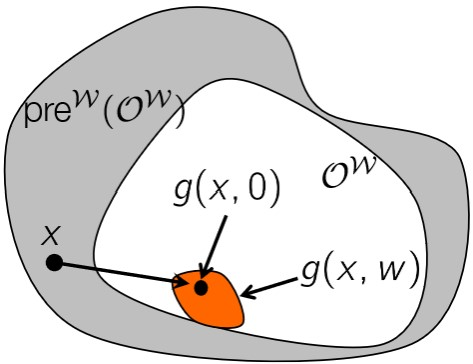
\includegraphics[width= 0.6\linewidth]{MPC_summary/Images/RPI.jpg}
        \end{center}
    \end{minipage}
    \subsubsection{Compute RPI sets}
    \textbf{Input: }$g,\mathcal{X,W}$\\
    \textbf{Output: }$\mathcal{O}^\mathcal{W}_\infty$\\
        $\hspace*{5mm} \Omega_0 \leftarrow \mathcal{X}$\\
         \hspace*{5mm}\textbf{loop}\\
         \hspace*{8mm}$\Omega_{i+1} \leftarrow \textrm{pre}^\mathcal{W}(\Omega_i) \cap\Omega_i$\\
         \hspace*{8mm}\textbf{if }$\Omega_{i+1} = \Omega_i$ \textbf{then}\\
         \hspace*{10mm}\textbf{return} $\mathcal{O} ^\mathcal{W}_\infty = \Omega_i$\\
         \hspace*{8mm}\textbf{end if}\\
         \hspace*{5mm}\textbf{end loop}\\
    \textbf{NOTE:} This is the same as for the nominal case, just $\mathrm{pre}(\Omega)$ replaced by $\mathrm{pre}^\mathcal{W}(\Omega)$
    \subsubsection{Robust Constraint Satisfaction}
    \begin{minipage}{0.2\linewidth}
        \begin{align*}
        \begin{rcases}
            \Phi_{i+1} &= A\Phi_i+Bu_i + w_i\\
            u_i &\in \mathcal{U}\\
            \Phi_i &\in \mathcal{X}\hspace{2mm}\forall W \in \mathcal{W}^N
        \end{rcases}
        \end{align*}
    \end{minipage}
    \begin{minipage}{0.5\linewidth}
         \begin{itemize}
             \item $i=0,\dots,N-1$
             \item Optimize over control action$\{u_0,\dots,u_{N-1}\}$
             \item Enforce constraints explicitly by imposing $\Phi_i\in\mathcal{X}$ and $u_i\in \mathcal{U}\forall$ sequences$W$.
         \end{itemize}
    \end{minipage}
    
     \begin{minipage}{0.23\linewidth}
        \begin{align*}
        \begin{rcases}
            \Phi_N &\in \mathcal{X}_f\\
            \Phi_{i+1} &= (A+BK)\Phi _i+w_i
        \end{rcases}
        \end{align*}
    \end{minipage}
    \begin{minipage}{0.5\linewidth}
         \begin{itemize}
             \item $i=N,\dots$
             \item Assume control law to be linear $u_i=K\Phi_i$
             \item Enforce constraints implicitly by imposing $\Phi_N$ to be in a robust invariant set $\mathcal{X}_\subseteq \mathcal{X}$ and $K\mathcal{X}_f \subseteq\mathcal{U}$ for the system $\Phi_{i+1} = (A+BK)\Phi_i+w_i$.
         \end{itemize}
    \end{minipage}
    \subsubsection{Pros vs. Cons}
\begin{minipage}[t]{0.65\linewidth}
\textbf{Pros} 
\begin{itemize}
    \item feasible set is invariant and we know exactly when controll will work 
    \item easier to tune: robustness vs. performance
\end{itemize}
\end{minipage}
\begin{minipage}[t]{0.3\linewidth}
\textbf{Cons}
\begin{itemize}
    \item complex, conservativ
    \item must know largest $W$
    \item feasible set small
    \end{itemize}
\end{minipage}
    \subsection{Set Operations}
    \textbf{Minkowski Sum:} Let $A$ and $B\subset\mathbb{R}^n$. 
    \[A\oplus B := \{x+y | x \in A,y\in B\}\]
    Add set $\mathcal{Y}$ to every point in $\mathcal{X}$\\
    \textbf{Pontryagin Difference:} Let $A$ and $B\subset\mathbb{R}^n$. 
     \[A\ominus B := \{x|x+e\in A \hspace{3mm}\forall e \in B\}\]
     \begin{center}
     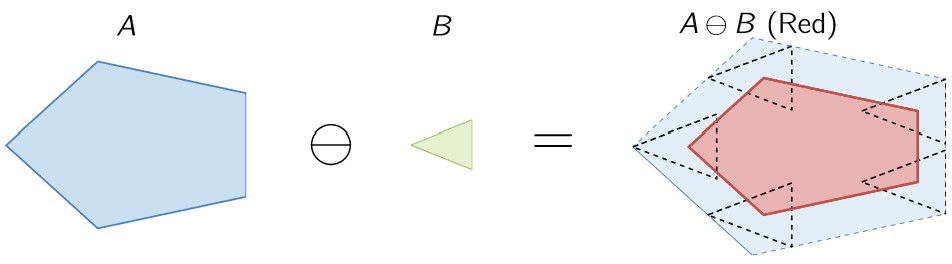
\includegraphics[width=0.7\linewidth]{MPC_summary/Images/PontryaginDiff.jpg}
     \end{center}
     Where we can add our $B$- set and is still fully contained in set $A$.
    \subsection{MPC as  a Game}
    Controller vs Disturbance
    \[x(k+1)= g(x(k),u(k))+w(k)\]
    \begin{itemize}
        \item Controller chooses his move $u$
        \item Disturbance decides on his move $w$ \textbf{after seeing the controller's move}
    \end{itemize}
    \textbf{Open-loop predictions:}
    \begin{itemize}
        \item Controller chooses a sequence of $N$ moves in the future $\{u_0,\dots, U_{N-1}\}$
        \item Disturbance chooses $N$ moves \textbf{knowing all} $N$ \textbf{moves of the controller}
    \end{itemize} 
    we are assuiming that the controller will do the same thing in the future no matter what the disturbance does!
    we can do better 
    \textbf{Closed-loop predictions}
    \begin{enumerate}
        \item Controller decides his first move $u_0$
        \item Disturbance chooses his first move $w_0$
        \item Controller decides his second move $u_1(x_1)$ \textbf{as a function of the first disturbance} $w_0$ \textbf{(recall $x_1=Ax_0+Bu_0+w_0$)}
        \item Disturbance chooses his second move $w_1$ as a function of $u_1$
        \item Controller decides his second move $u_2(x_2)$ \textbf{as a function of the first two disturbances} $w_0, w_1$
    \end{enumerate}
    \subsection{Closed Loop MPC}
    \textbf{Pre-stabilization} $\mu_i(x_i) = Kx_i + v_i$
    \begin{itemize}
        \item Fixed K, such that A+BK is stable
        \item simple, often conservative
    \end{itemize}
    \textbf{Linear feedback}$\mu_ui(x_i) = K_i x_i + v_i$
    \begin{itemize}
        \item Optimize over $K_i$ and $v_i$
        \item Non-convex difficult to solve
    \end{itemize}
    \textbf{Disturbance feedback }$\mu_i(x_i) =\sum^{i-1}_{j=0}M_{ij}w_j+v_i$
    \begin{itemize}
        \item Optimize over $M_{ij}$ and $v_i$
        \item Equivalent to linear feedback, but convex!
        \item Can be very effective, but computationally intense.
    \end{itemize}
    \textbf{Tube-MPC} $\mu_i(x_i) = v_i +K(x_i-\Bar{x}_i$  
        \begin{itemize}
            \item Fixed $ K$ such that $A+BK$ is stable
            \item Optimize voer $\Bar{x}_i$ and $v_i$
            \item Simple, and can be effective
        \end{itemize}
\subsection{Tube MPC}
\subsubsection{The Idea}
seperate the available control authority into two parts
\begin{enumerate}
    \item A portion that steers the noise free 'nominal' system to the origin $z(k+1) = Az(k)+Bv(k)$
    \item A portion that compensates for deviations from this system, i.e a 'tracking' controller, to keep the real trajectory close to the nominal
    \[u_i=K(x_i-z_i)+v_i\]
    for some linear controller $K$ offline, and optimize over the nominal trajectory$\{v_0,\dots,v_{N-1}\}$ which results in a convex problem.
\end{enumerate}
\subsection{Procedure}
\begin{enumerate}
    \item Computing set $\epsilon$ thet error will remain inside
    \item Modify constraints on nominal trajectory $\{z_i\}$ s.th. $z_i \oplus \epsilon \subset \mathcal{X} and v_i \in \mathcal{U} \ominus K \epsilon$
    \item Formulate as convex optimization problem, prove constraints and stability
\end{enumerate}
\subsubsection{Part 1) Minimum robust invariant set $\epsilon$ (mRPI)}
\begin{itemize}
    \item Robust constraint satisfaction: max robust invariant set
    \item Now the \textbf{mRPI} neede, in which states will remain inside despite the noise.
    \item For the system $x_{i+1} = Ax_i + w_i$ with $\mathbf{x_0 = 0}$, the saae evolution is $x_i = \sum^{i-1}_{j=0}A^jw_{i-1-j}$
    \item Set containing all possible states $x_i$ is $F_i = \oplus^{i-1}_{j=0} A^jW,F_o = \{0\}$\\
    $\Rightarrow$ \textbf{mRPI:} $F_\infty = \oplus^\infty_{j=0}A^jW$ and if $\exists n $s.th. $F_n = F_{n+1}$ then $F_n = F_\infty$
    \item \textbf{Note:} in closed loop $A = A+BK$ if $u=Kx$
\end{itemize}
\subsubsection{Part 2) Modify Constraints: tightening}
Given nominal trajectory $z_i$, the error $e_i$ will be in the set $\epsilon
$, so the noisy system trajectory $x_i+z_i +e_i$ can only be up to $\epsilon$ far away from $z_i$:
\[x\in z_i \oplus \epsilon = \{z_i+e|e \in \epsilon\}\]
$\Rightarrow$ sufficient condition: $z_i \in \mathcal{X} \ominus\epsilon \Rightarrow x_i \in z_i \oplus\epsilon \subseteq \mathcal{X}$ $\epsilon$ is known offline and constrains $\mathcal{X}\ominus \epsilon$ can also be computed offline\\
$\Rightarrow$ condition for input $v_i \in \mathcal{U} \ominus K \epsilon \Rightarrow u_i \in K \epsilon \oplus v_i \subset \mathcal{U}$\\
\textbf{Tightening for Polytopic Constraints}
\begin{itemize}
    \item \textbf{State: } $Fx_i \leq f \Leftrightarrow Fz_i + Fe_i \leq f \forall e_i \in \epsilon \Leftrightarrow Fz_i \leq f - \underset{e_i\in\epsilon}{\textrm{max }}Fe_i$
    \item \textbf{Input: } $Hu_i \leq h \Leftrightarrow Hv_i + HKe_i\leq h \forall e_i \in \epsilon \Leftrightarrow H v_i \leq h - \underset{e_i\in\epsilon}{\textrm{max }} HK e_i$
\end{itemize}
\subsubsection{Part 3) convex Optimization Formulation}
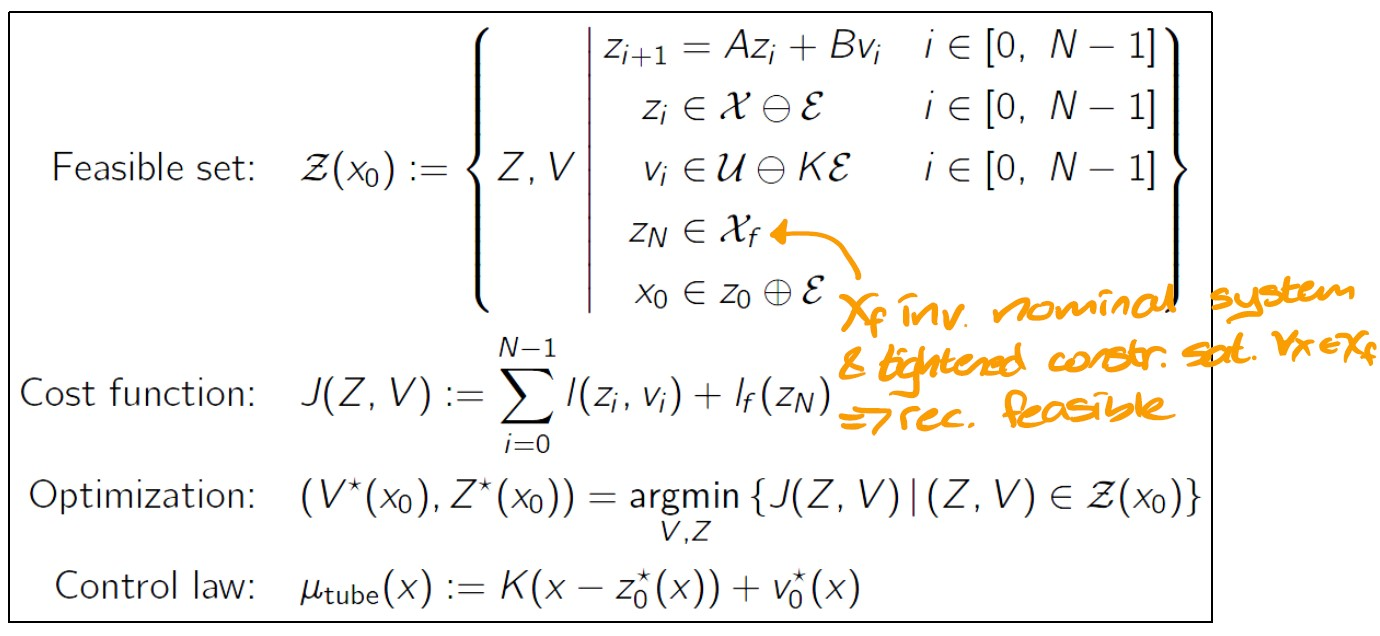
\includegraphics[width=0.99\linewidth]{MPC_summary/Images/Convex_optmization.jpg}
\begin{itemize}
    \item Optimizing nominal system with tightend state \& input constraints
    \item First tube centre is optimization variable $\rightarrow$ must be within $\epsilon$ of $x_0$
    \item Cost w.r.t tube centres (nom. system) and terminal set w.r.t. tightened constraint
\end{itemize}
\subsubsection{Error Dynamics}
\begin{itemize}
    \item \textbf{Error:} $e_i = x_i-z_i$ which gives the error dynamics:
        \begin{align*}
            e_{i+1} &= x_{i+1}-z_{i+1}\\
            &= Ax_i+Bu_i +w_i - Az_i -Bv_i\\
            &= Ax_i +BK(x_I-z_i)+Bv_i+w_i -Az_i-Bv_i\\
            &=(A+BK)(x_i-z_i)+w_i\\
            &=(A+BK)e_i+w_i
        \end{align*}
    \item Bound maximum error, $\rightarrow$ bound real trajectory deviation from nominal
        \[e_{i+1} = (A+BK)e_i+w_i \hspace{4mm} w_i\in \mathcal{W}\]
\end{itemize}

Dynamics $A+BK$ are stable , and the set $\mathcal{W}$ is bounded, so there is some set $\epsilon$ that $e$ will stay inside for all time. We want the smallest such set (the 'minimal robust invariant set')
\subsubsection{How to}
\begin{itemize}
    \item Compute the set $\mathbf{\varepsilon}$ that the error will remain inside $\rightarrow$ \textbf{minimum} robust invariant set $\rightarrow$ the smallest set that the state will remain inside despite the noise.
   
    \item Modify constraints on nominal trajectory $\{z_i\}$ so that $z_i\oplus\varepsilon\subset\mathcal{X}$ and $v_i \in \mathcal{U}\ominus K\varepsilon$
    \item Formulate as convex optimization problem
    \item prove that constraints are robustly satisfied
     \item The closed loop system is robustly stable
\end{itemize}
\subsubsection{Uncertain State Evolution}
Consider the system $x_{i+1} = Ax_i+w_i$ and assume that $x_0=0$ how close can we stay to the origin?
 \begin{align*}
     x_1 &= w_0\\
     x_2 &= Ax_1+w_1=Aw_0+w_1\\
     \vdots\\
     x_i &= \sum^{i-1}_k=0 A^kw_{i-1-k}
 \end{align*}
 Assume that $w_i\in\mathcal{W}\forall i$ the set $F_i$ that contains all possilbe states $x_i$ \[F_i=\mathcal{W}\oplus A\mathcal{W}\dots\oplus A^{i-1}\mathcal{W}=\bigoplus^{i-1}_{j=0}A^j\mathcal{W}, F_0 := \{0\}\]
With increasing $i$ we arrive at the \textbf{minimum robust invariant set} mRPI \[F_\infty=\bigoplus^\infty_{j=0}A^j\mathcal{W}, \hspace{5mm} F_0 := \{0\}\]
\subsubsection{Pseudocode}
\begin{minipage}{0.4\linewidth}
\textbf{Input:} $A$ \\
\textbf{Output:} $ F_\infty $ \\
\hspace*{3mm} $\Omega_0 \leftarrow \{0\}$\\
\hspace*{3mm} \textbf{loop}\\
\hspace*{5mm} $\Omega_{i+1} \leftarrow \Omega_i \oplus A^i \mathcal{W}$\\
\hspace*{5mm} \textbf{if} $\Omega_{i+1} = \Omega_i$ \textbf{then}\\
\hspace*{8mm} \textbf{return} $F_\infty=\Omega_i$\\
\hspace*{5mm} \textbf{end if}\\
\hspace*{3mm} \textbf{end loop}
\end{minipage}
\begin{minipage}{0.5\linewidth}
\begin{itemize}
    \item A finite $n$ does not always exist, but a 'large' $n$ is a good approximation
    \item if $n$ is not finite, there are other methods of computing small invariant sets, which will be slightly larger than $F_\infty$
\end{itemize}
\end{minipage}
\subsubsection{To implement tube MPC}
\textbf{Offline:}
\begin{enumerate}
    \item Choose a stabilizing controller $K$ so that $||A+BK||<1$
    \item Compute the minimal robust invariant set $\varepsilon = F_\infty$ for the system $x(k+1) = (A+BK)x(k) + w(k), w \in\mathcal{W}^1$
    \item Compute the tightened constraints $\Tilde{\mathcal{X}}:=\mathcal{X} \ominus \varepsilon, \Tilde{\mathcal{U}}:= \mathcal{U} \ominus K\varepsilon$
    \item Choose terminal weight function $I_f$ and constraint $\mathcal{X}_f$ satisfying assumption \[I_f(Az+B_{\mathcal{K}_f}(z)) -I_f(z)  \leq -I(z,\mathcal{K}_f(z))\forall z \in \mathcal{X}_f\]
\end{enumerate}
\textbf{Online}
\begin{enumerate}
    \item Measure / estimate state $x$
    \item Solve the problem $(V^*(x),Z^*(x)) =\underset{V,Z}{\mathrm{argmin}}\{J(Z,V)|(Z,V)\in \mathcal{Z}(x)\}$
    \item set the input to $u=K(x-z_0^*(x))+v_0^*(x)$
\end{enumerate}
\subsubsection{Pros vs. Cons}
\begin{minipage}[t]{0.65\linewidth}
\textbf{Pros} 
\begin{itemize}
    \item less conservative than open loop robust MPC(actively compensating noise)\\
    \item Works for unstable systems, optimizatoin simple
\end{itemize}
\end{minipage}
\begin{minipage}[t]{0.3\linewidth}
\textbf{Cons}
\begin{itemize}
    \item sub-optimal MPC
    \item reduce feasible set
    \item $W$ not known exactly
\end{itemize}
\end{minipage}
\subsection{Nominal MPC with Noise}
to control the noisy system \[x(k+1) = Ax(k)+Bu(k)+w(k)\]
\subsection{Input to State Stability ISS}
\begin{center}
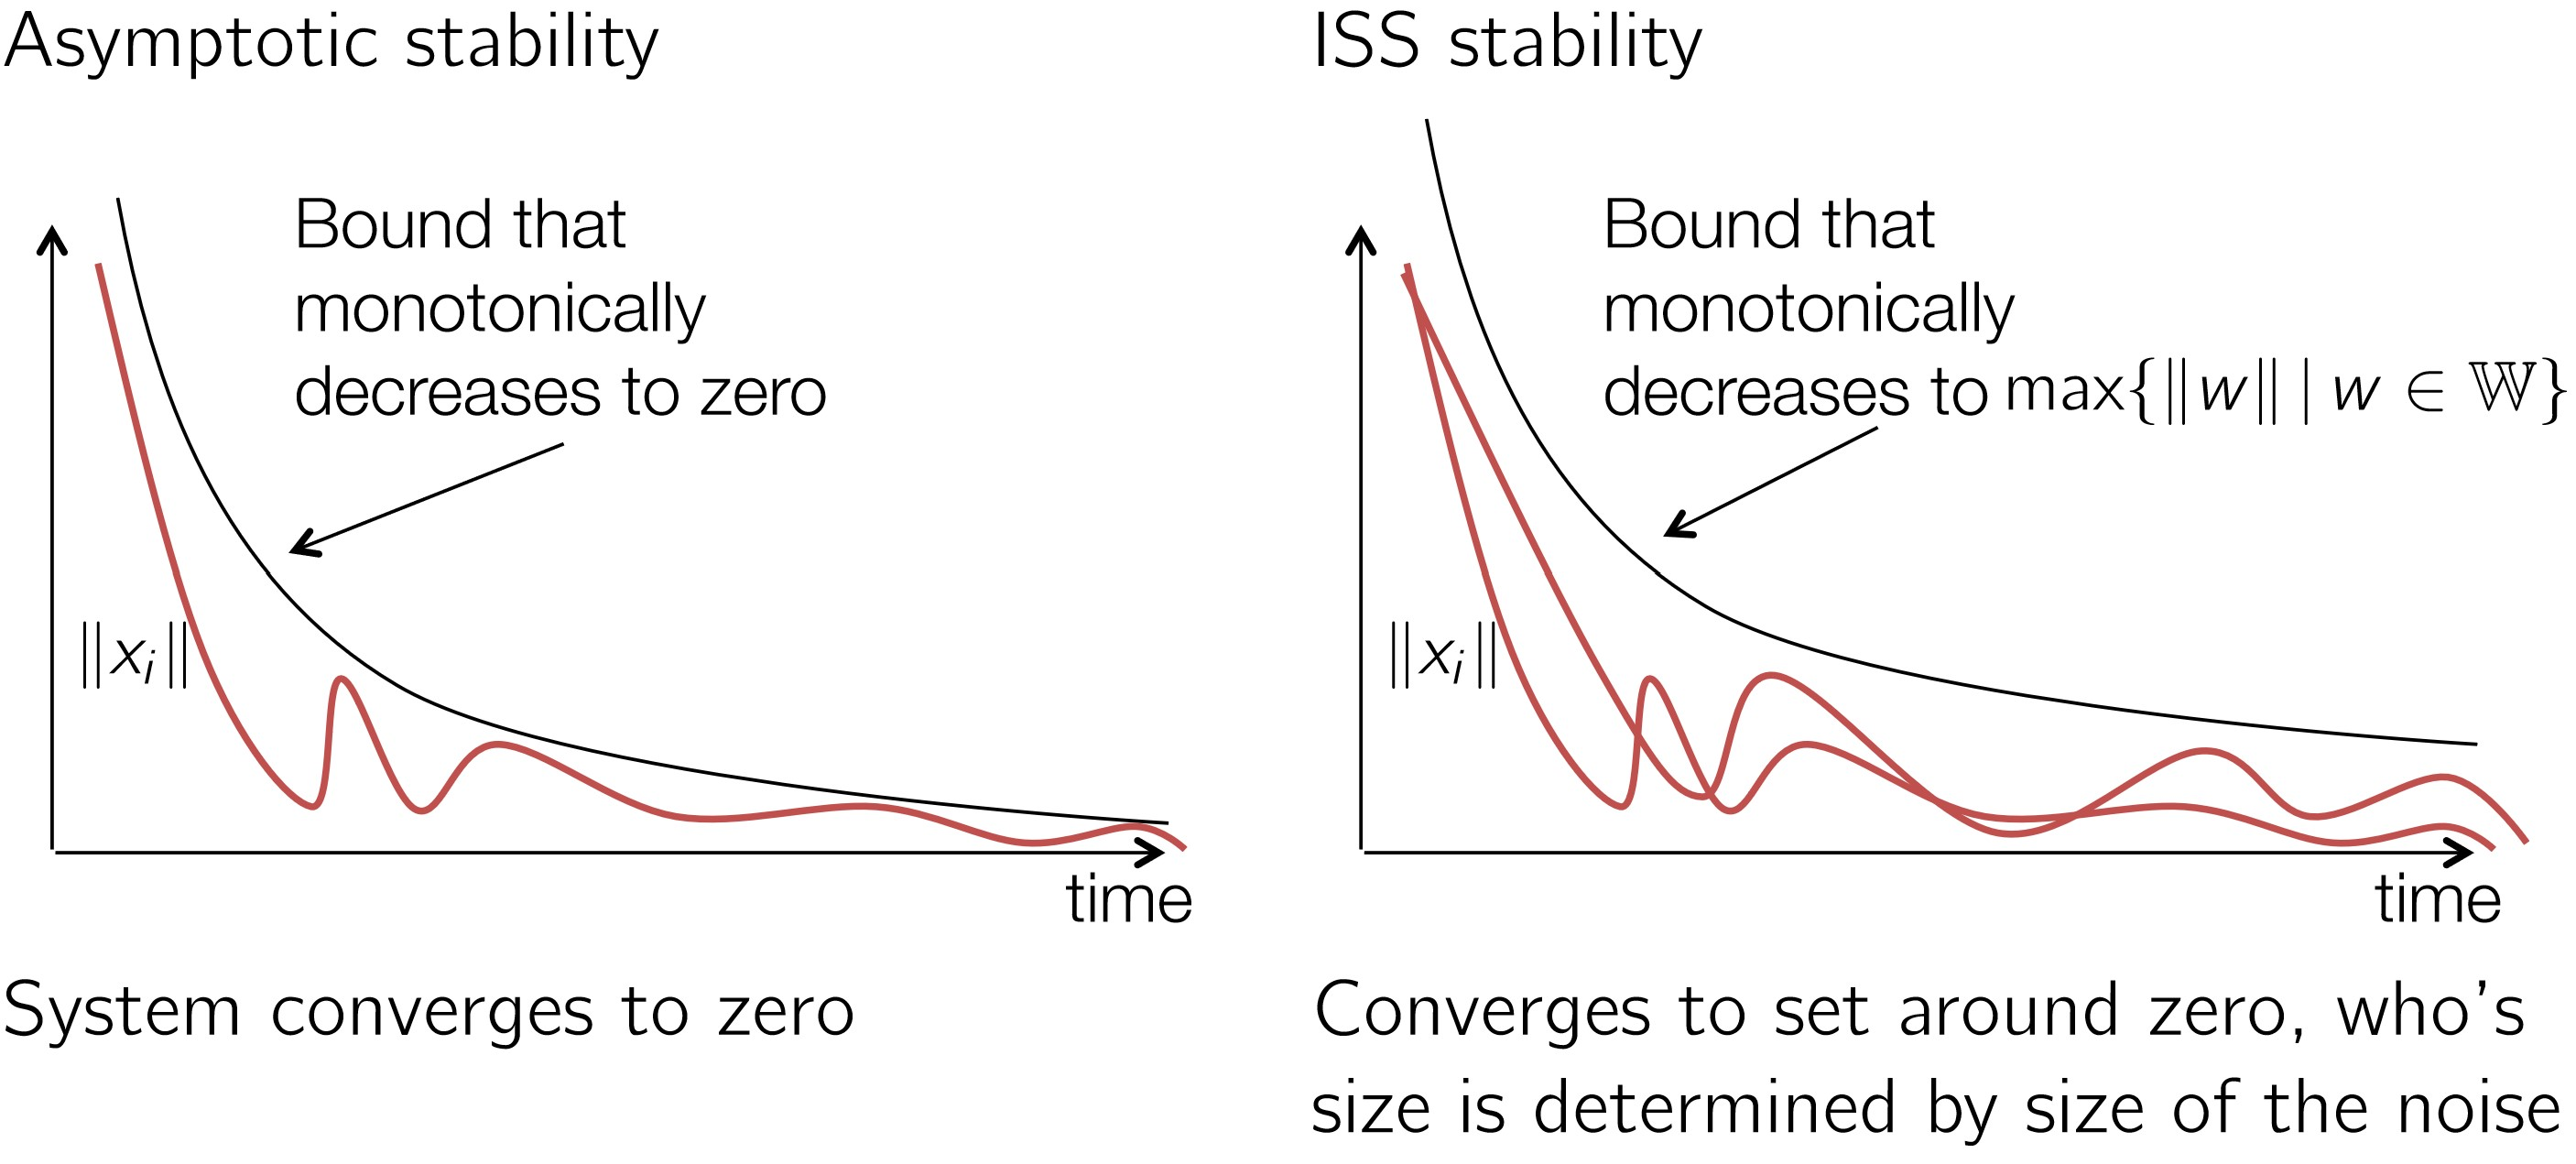
\includegraphics[width=0.7\linewidth]{MPC_summary/Images/Asymptotic_stability_ISS.jpg}
\end{center}